%%%%%%%%%%%%%%%%%%%%%%%%%%%%%%%%%%%%%%%%%%%%%%%%%%%%%%%%%%%%%%%%%%%%%%%%%%%%%
% AMEE 2026 Abstract Submission
% Theme: Patient Safety
% Web-Based Interactive CCU Orientation Manual
%%%%%%%%%%%%%%%%%%%%%%%%%%%%%%%%%%%%%%%%%%%%%%%%%%%%%%%%%%%%%%%%%%%%%%%%%%%%%

\documentclass[11pt,a4paper]{article}

% Packages
\usepackage[utf8]{inputenc}
\usepackage[T1]{fontenc}
\usepackage{helvet}
\usepackage[margin=2.5cm]{geometry}
\usepackage{xcolor}
\usepackage{titlesec}
\usepackage{enumitem}
\usepackage{hyperref}
\usepackage{fancyhdr}
\usepackage{graphicx}
\usepackage{tikz}

% Colors
\definecolor{navyblue}{RGB}{26,54,93}
\definecolor{lightblue}{RGB}{49,130,206}
\definecolor{coral}{RGB}{229,62,62}
\definecolor{success}{RGB}{56,161,105}
\definecolor{textgray}{RGB}{100,116,139}

% Sans-serif font
\renewcommand{\familydefault}{\sfdefault}

% Section formatting
\titleformat{\section}{\large\bfseries\color{navyblue}}{\thesection}{0em}{}[\vspace{-0.5em}\color{navyblue}\hrule\vspace{0.5em}]
\titleformat{\subsection}{\normalsize\bfseries\color{lightblue}}{\thesubsection}{0em}{}

% Header/Footer
\pagestyle{fancy}
\fancyhf{}
\fancyhead[L]{\small\color{textgray}AMEE 2026 Abstract Submission}
\fancyhead[R]{\small\color{textgray}Patient Safety Theme}
\fancyfoot[C]{\small\color{textgray}\thepage}
\renewcommand{\headrulewidth}{0.5pt}
\renewcommand{\footrulewidth}{0pt}

% Hyperref setup
\hypersetup{
    colorlinks=true,
    linkcolor=lightblue,
    urlcolor=lightblue,
    citecolor=lightblue
}

\begin{document}

%----------------------------------------------------------------------
% HEADER
%----------------------------------------------------------------------
\begin{center}
    \colorbox{navyblue}{%
        \parbox{0.95\textwidth}{%
            \centering
            \vspace{0.8em}
            {\Large\bfseries\color{white}AMEE 2026 ABSTRACT SUBMISSION}\\[0.3em]
            {\normalsize\color{white}The AMEE Conference 2026 $\bullet$ Vienna, Austria $\bullet$ August 22--26, 2026}\\[0.3em]
            \vspace{0.5em}
        }%
    }
\end{center}

\vspace{1em}

%----------------------------------------------------------------------
% THEME AND PRESENTATION TYPE
%----------------------------------------------------------------------
\begin{center}
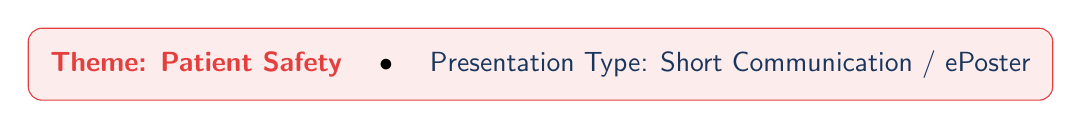
\begin{tikzpicture}
    \node[rectangle, draw=coral, fill=coral!10, rounded corners=5pt, inner sep=8pt] {
        \textcolor{coral}{\textbf{Theme: Patient Safety}} \quad $\bullet$ \quad
        \textcolor{navyblue}{Presentation Type: Short Communication / ePoster}
    };
\end{tikzpicture}
\end{center}

\vspace{1.5em}

%----------------------------------------------------------------------
% TITLE
%----------------------------------------------------------------------
\section*{TITLE}

{\Large\bfseries\color{navyblue}
Web-Based Interactive CCU Orientation Manual: Eliminating Arterial Line-Related Compartment Syndrome Through Digital Education
}

\vspace{0.3em}
{\small\color{textgray}(18 words)}

\vspace{1.5em}

%----------------------------------------------------------------------
% AUTHORS
%----------------------------------------------------------------------
\section*{AUTHORS}

\begin{enumerate}[leftmargin=2em, itemsep=0.8em]
    \item \textbf{Mu-Yang Hsieh, MD, PhD, FESC} \hfill \colorbox{success!20}{\small\textcolor{success}{\textbf{Presenter}}}\\
    {\small Division of Cardiology, National Taiwan University Hospital Hsinchu Branch\\
    Hsinchu, Taiwan\\
    Email: \href{mailto:muhsieh@ntuh.gov.tw}{muhsieh@ntuh.gov.tw}}

    \item \textbf{Chen-Wei Lien, MD}\\
    {\small Division of Cardiology, National Taiwan University Hospital Hsinchu Branch\\
    Hsinchu, Taiwan}

    \item \textbf{Ru-Ying Hsu, MD}\\
    {\small Division of Cardiology, National Taiwan University Hospital Hsinchu Branch\\
    Hsinchu, Taiwan}

    \item \textbf{Li-Ta Keng, MD}\\
    {\small Division of Pulmonology, National Taiwan University Hospital Hsinchu Branch\\
    Hsinchu, Taiwan}

    \item \textbf{Ming-Hsien Lee, RN}\\
    {\small Department of Nursing, National Taiwan University Hospital Hsinchu Branch\\
    Hsinchu, Taiwan\\
    Email: \href{mailto:mekennlee@gmail.com}{mekennlee@gmail.com}}
\end{enumerate}

\vspace{1.5em}

%----------------------------------------------------------------------
% ABSTRACT
%----------------------------------------------------------------------
\section*{ABSTRACT}

{\small\color{textgray}Word count: 347 / 350 words (excluding title and author details)}

\vspace{1em}

\subsection*{BACKGROUND}
Arterial line placement is a routine procedure in coronary care units (CCU), yet poses significant bleeding risks for acute myocardial infarction (AMI) patients receiving dual antiplatelet therapy (DAPT) combined with anticoagulation. Between 2022--2025, our 10-bed CCU experienced five cases of brachial artery puncture-related compartment syndrome requiring emergency fasciotomy. Root cause analysis using the Human Factors Analysis and Classification System (HFACS) identified critical gaps: absence of standardized arterial line placement guidelines, inadequate risk stratification for anticoagulated patients, and insufficient education on DAPT bleeding complications.

\subsection*{SUMMARY OF WORK}
We developed a comprehensive web-based CCU orientation manual as an educational intervention. This React-based single-page application features nine interactive modules: daily checklists, safety case studies (including the compartment syndrome cases), ACS medication orders, heart failure certification workflows, special post-procedure care protocols, drug reference tables, emergency algorithms, chart writing guides, and self-assessment quizzes. The intervention specifically embedded: (1) new arterial line placement guidelines prioritizing radial artery with ultrasound guidance, (2) explicit prohibition of brachial artery puncture in patients on Brilinta/Prasugrel, and (3) standardized 6P monitoring protocol (Pain, Paralysis, Pallor, Polar, Paresthesia, Pulseless) post-procedure. The manual was deployed in September 2025 as mandatory orientation material for all CCU residents and nurse practitioners.

\subsection*{SUMMARY OF RESULTS}
Following implementation, we achieved zero arterial line-related compartment syndrome cases over six months of monitoring (August 2025--January 2026), representing a \textbf{\textcolor{success}{100\% reduction}} from the previous incidence of 1.6 cases/year. Secondary outcomes demonstrated improvement: radial artery first-choice rate increased from 65\% to 95\%, ultrasound-guided puncture rate rose from 40\% to 90\%, 6P monitoring protocol compliance reached 100\%, and 92\% of learners achieved passing scores ($\geq$80\%) on the integrated knowledge assessment quiz.

\subsection*{DISCUSSION AND CONCLUSIONS}
This quality improvement initiative demonstrates that HFACS-driven root cause analysis, combined with web-based interactive educational tools, can effectively eliminate preventable procedural complications. The just-in-time accessibility, interactive case-based learning, and integrated self-assessment features of digital education platforms offer advantages over traditional orientation methods.

\subsection*{TAKE-HOME MESSAGES}
\begin{enumerate}[leftmargin=2em, itemsep=0.3em]
    \item Web-based interactive education effectively reduces high-risk procedural complications
    \item HFACS framework enables systematic identification of educational gaps in patient safety
    \item Digital orientation manuals provide accessible, updateable just-in-time learning resources
\end{enumerate}

\vspace{1.5em}

%----------------------------------------------------------------------
% KEYWORDS
%----------------------------------------------------------------------
\noindent\textbf{\color{navyblue}Keywords:} Patient safety, Digital education, Compartment syndrome, HFACS, Quality improvement, Coronary care unit, Procedural complications

\vspace{2em}

%----------------------------------------------------------------------
% SUBMISSION INFO
%----------------------------------------------------------------------
\begin{center}
\colorbox{lightblue!10}{%
    \parbox{0.9\textwidth}{%
        \centering
        \vspace{0.8em}
        {\bfseries\color{navyblue}SUBMISSION INFORMATION}\\[0.5em]
        \begin{tabular}{rl}
            \textbf{Theme:} & Patient Safety \\
            \textbf{Word Count:} & 347 words (limit: 350) \\
            \textbf{Title Words:} & 18 words (limit: 20) \\
            \textbf{Deadline:} & January 19, 2026 \\
            \textbf{Submit at:} & \href{https://amee.org/events/amee-2026/abstract-submissions/}{amee.org/events/amee-2026/abstract-submissions/}
        \end{tabular}
        \vspace{0.8em}
    }%
}
\end{center}

\end{document}
